\documentclass[11pt,a4paper]{article}
\usepackage[margin=2.2cm]{geometry}
\usepackage{booktabs,amsmath,hyperref,xcolor,enumitem,tikz}
\usetikzlibrary{arrows.meta,positioning}
\hypersetup{colorlinks,linkcolor=blue!50!black,urlcolor=blue!50!black,citecolor=blue!50!black}
\setlist{itemsep=1pt,topsep=3pt}
\title{\textbf{CrackDistill: Distilling SAM\,2 into YOLOv11n-seg for Crack Segmentation}\\[2pt]
\large Progress report (June--October 2026), findings, and next architectures}
\author{Shahin Alakbarov}
\date{28 October 2026}
\begin{document}
\maketitle

\begin{abstract}
We distil the Segment Anything Model~2 (SAM\,2.1 Hiera-Large, 224M parameters) into a 2.84M-parameter
YOLOv11n-seg student for pavement-crack instance segmentation on Crack500. Over five months (79 commits) the
project went from early KD ``gains'' to a corrected, controlled protocol. After fixing several silent bugs
(teacher misalignment of about 140\,px, wrong instance pairing for 58\% of pairs, a baseline that still
received KD loss), we find that \textbf{the KD gain seen without augmentation (+0.053 mask mAP50) disappears once the
baseline is properly augmented}. Flips and rotations alone add +0.104, and standard YOLO augmentation is best
overall (val mask mAP50 0.540; test pixel F1 0.731 on crops, 0.707 on full photos). A data-efficiency study
(50\% of the data) also shows no KD benefit. We review 2023--2026 literature and propose next steps: a better
teacher (crack-fine-tuned SAM), SAM\,1+SAM\,2 logit fusion with standardisation, and KD schedules.
\end{abstract}

\section{Goal and setup}
\begin{itemize}
\item \textbf{Task:} crack instance segmentation; a real-time student for edge devices.
\item \textbf{Teacher:} SAM\,2.1 Hiera-L, prompted with each ground-truth crack's box. Pre-sigmoid mask logits are
cached offline as \texttt{M$\times$256$\times$256} per image (2,196 files).
\item \textbf{Student:} YOLOv11n-seg (2.84M parameters; 10.8\,ms per 512 tile on a T4). It beat YOLOv8n-seg in early tests (0.540 vs 0.532).
\item \textbf{Data:} Crack500, official split (1,896 / 348 / 1,124 crops; 200 full test photos).
\item \textbf{KD loss:} the task loss plus a temperature-scaled Bernoulli KL between student mask logits and the
teacher logits, warped into the student's letterboxed frame.
\end{itemize}

\begin{center}
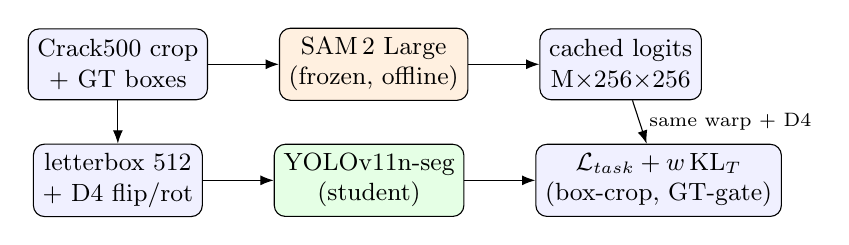
\begin{tikzpicture}[node distance=0.55cm and 0.9cm, every node/.style={font=\small},
 box/.style={draw,rounded corners,align=center,minimum height=0.9cm,fill=blue!6}]
\node[box] (img) {Crack500 crop\\+ GT boxes};
\node[box,right=of img,fill=orange!12] (sam) {SAM\,2 Large\\(frozen, offline)};
\node[box,right=of sam] (cache) {cached logits\\M$\times$256$\times$256};
\node[box,below=of img] (aug) {letterbox 512\\+ D4 flip/rot};
\node[box,right=of aug,fill=green!10] (yolo) {YOLOv11n-seg\\(student)};
\node[box,right=of yolo] (loss) {$\mathcal{L}_{task}+w\,\mathrm{KL}_T$\\(box-crop, GT-gate)};
\draw[-Latex] (img)--(sam); \draw[-Latex] (sam)--(cache);
\draw[-Latex] (img)--(aug); \draw[-Latex] (aug)--(yolo); \draw[-Latex] (yolo)--(loss);
\draw[-Latex] (cache)--node[right,font=\scriptsize]{same warp + D4}(loss);
\end{tikzpicture}
\end{center}

\section{Evolution of the project}
\begin{description}
\item[P0 (Jun--mid Jul).] SAM\,2 logits cached (15 Jun). First YOLOv8 KD notebooks; FP16 NaN in the KD loss fixed by clamping.
\item[P1 (20 Jul--4 Aug).] Repository created. Optuna tuned the loss weights ($T{=}3.78$, $w_{mask}{=}0.96$). Box and box+centroid prompts gave identical results. YOLOv11n chosen as the student.
\item[P2 (5--14 Aug).] Ablations: mask-KL was the useful term and feature MSE hurt. We found that some KD notebooks had \emph{never loaded teacher logits}; every run now prints a logit-file count.
\item[P3 (15 Aug--11 Sep).] Many variants: dilated, affinity, multi-scale, channel-wise feature KD (CWD), Tversky, two-stage, out-of-distribution tiling. All scored 0.53--0.55 mask mAP50, and a 21-page draft was written. These numbers were later invalidated.
\item[P4 (16--29 Sep): scientific audit.] Bugs found and fixed:
 \begin{itemize}
 \item the training-time letterbox pad was read as 0.8\,px instead of 112\,px, so the teacher sat about 140\,px off the crack;
 \item \texttt{overlap\_mask} reordered instances, so only 42\% of teacher--student pairs were correct (99.9\% after the fix);
 \item the ``clean'' baseline still received the KD loss;
 \item the baseline had augmentation and the KD arms did not;
 \item the GT-soft control actually used SAM logits;
 \item EXIF rotation was handled wrongly (130 of 200 test photos);
 \item the seed was not passed to Ultralytics, feature hooks sat on the wrong layers, and the Kaggle dataset linker was ambiguous.
 \end{itemize}
 The measured SAM-vs-GT median IoU is 0.605.
\item[P5 (early Oct): v1 protocol, no spatial augmentation.] Baseline 0.410, Mask-KD 0.463, GT-soft 0.414. Every arm overfit (best epoch 9--17).
\item[P6 (14 Oct): v2 design.] Augmentation-consistent KD: the cached teacher map receives the same D4 flip/rotation as the image. Our measurements showed the crack fills only 0.9\% of the KD canvas and SAM recalls only 56\% of cracks 4\,px wide or thinner, which motivated a new box-cropped, GT-gated KL (A5). The feature, boundary and affinity losses were dropped.
\item[P7 (24 Oct): Stage A] and \textbf{P8 (28 Oct): data-efficiency}, below.
\end{description}

\section{Results}
\begin{table}[h]\centering\small
\caption{Stage A, seed 0, Kaggle T4, 150 epochs. Val = 348 crops; test = scale-matched evaluator (thresholds tuned on val).}
\begin{tabular}{lcccc}
\toprule
Arm & val mask mAP50 & test crops F1 & 200 full photos F1 & T4 time\\
\midrule
v1 baseline (no spatial aug.) & 0.410 & -- & -- & 1.2\,h\\
v1 Mask-KD (no spatial aug.) & 0.463 & -- & -- & 2.0\,h\\
\midrule
A1 baseline + D4 & 0.514 & 0.713 & 0.684 & 1.4\,h\\
A2 Mask-KD + D4 & 0.503 & -- & -- & 2.0\,h\\
A3 GT-soft control + D4 & 0.481 & -- & -- & 2.4\,h\\
A5 gated Mask-KD + D4 & 0.511 & 0.704 & 0.661 & 2.6\,h\\
\textbf{A4 baseline + YOLO default aug.} & \textbf{0.540} & \textbf{0.731} & \textbf{0.707} & 1.4\,h\\
\bottomrule
\end{tabular}
\end{table}

\begin{table}[h]\centering\small
\caption{Data efficiency (val mask mAP50). Nested whole-photo subsets, identical for both arms.}
\begin{tabular}{lccc}
\toprule
Training data & Baseline (D4) & Gated KD (D4) & $\Delta$\\
\midrule
25\% (478 crops) & 0.454 & pending (rerun) & --\\
50\% (931 crops) & 0.502 & 0.482 & $-0.020$\\
100\% (1,896 crops) & 0.514 & 0.511 & $-0.003$\\
\bottomrule
\end{tabular}
\end{table}

\paragraph{Findings.}
\begin{enumerate}
\item \textbf{The v1 KD gain was a substitute for augmentation.} D4 alone added +0.104, twice the KD gain, and KD added nothing on top.
\item \textbf{SAM is a noisy teacher on thin cracks.} It misses 44\% of thin-crack pixels, and 21\% of its crack pixels are ground-truth background.
\item \textbf{Full photos must be tested at the training scale.} With an older checkpoint, ${\times}0.8$ tiling scored F1 0.71 against 0.60 when the whole photo was squeezed into 512\,px.
\item \textbf{Deliverable model:} A4, with 2.84M parameters and about 11\,ms per tile.
\end{enumerate}
Limitation: one seed so far. The claim is ``no gain'', not ``harm''.

\section{Diagnosis: the zero-shot teacher problem}
Knowledge distillation only helps when the teacher knows something the student cannot learn from the labels. Our measurements show that zero-shot SAM\,2 does not:
\begin{itemize}
\item \textbf{The teacher is worse than the labels.} SAM\,2 against the ground truth: median IoU 0.605. Recall is 0.56 on cracks 4\,px wide or thinner, and 21\% of its crack pixels are ground-truth background.
\item \textbf{The student alone already reaches pixel F1 0.71--0.73.} A teacher that is not clearly better only adds noise or label smoothing. The GT-soft control (A3) behaves the same way.
\item \textbf{The KD gain was really augmentation.} v1 KD gave +0.053 without spatial augmentation. Flips and rotations alone gave +0.104, and KD then added nothing.
\item \textbf{The cached teacher cannot follow mosaic or scale augmentation}, which is exactly where the best model (A4) gains.
\item \textbf{Fusing two zero-shot teachers (SAM\,1+SAM\,2) is unlikely to help by itself.} Both are prompted with the same boxes and both miss thin cracks, so their errors are correlated.
\end{itemize}
\textbf{Implication:} the bottleneck is the teacher's quality, not the KD loss. The teacher must first be made better than
the student, for example a crack-fine-tuned SAM with val pixel F1 above 0.80. Alternatively, it should be used where no labels exist (pseudo-labelling unlabelled images).

\section{Paper positioning}
The work done so far supports a paper whichever way the next experiments go:
\begin{itemize}
\item \textbf{Negative result (already supported).} ``Zero-shot foundation-model KD gains on a tiny crack segmenter
are an artefact of weak baselines.'' Evidence: the audit and its bug list (\S2), the GT-soft control, matched augmentation, the
data-efficiency curve, and scale-matched full-photo evaluation. Many KD papers compare against unaugmented baselines,
as our own v1 did, so this is a useful and honest contribution. What it still needs: 3 seeds and the 25\% point.
\item \textbf{Positive result (target).} ``A crack-tuned SAM teacher with semi-supervised distillation improves a 2.8M-parameter
segmenter beyond strong augmentation.'' Requirement, fixed in advance: beat A4 by at least 0.02 on val and test, over 3 seeds.
\item \textbf{Either way:} also report out-of-distribution results (DeepCrack, CFD), where a foundation-model teacher may help
generalisation even without an in-domain gain.
\end{itemize}

\section{Related work (2023--2026) and what it implies}
\begin{itemize}
\item \textbf{SAM is a noisy teacher on thin structures.} Boxes2Pixels~\cite{b2p} uses box-prompted SAM masks for defects and adds online
self-correction for SAM's false negatives (+9.7 binary IoU). SAMRefiner~\cite{samrefiner} cleans SAM pseudo-masks (+10\%).
CoGenSAM~\cite{cogen} and SERD~\cite{serd} report that raw SAM masks drop or over-segment cracks, and that SAM's internal
response keeps more crack pixels than its final masks (recall 82.7\% vs 74.7\%).
\item \textbf{A better teacher.} CrackSAM~\cite{cracksam} (adapter/LoRA), Segment Any Crack~\cite{sac} (fine-tuning only the normalisation layers), and
SAM2-Adapter~\cite{sam2ad} and SECrackSeg~\cite{secrack} all fine-tune SAM for cracks. A crack-tuned teacher is the most likely route to a real gain.
\item \textbf{Multi-teacher fusion.} Logit standardisation~\cite{logitstd} z-scores each teacher's logits, which is needed before averaging SAM\,1 and SAM\,2.
Adaptive per-pixel teacher weights for segmentation~\cite{adamt}. AM-RADIO~\cite{radio} uses a separate head per teacher instead of averaging.
TOM~\cite{tom} distils several teachers, including SAM, into one student. DIST~\cite{dist} handles a large teacher--student capacity gap.
\item \textbf{KD and augmentation.} The teacher must be consistent with the augmented view~\cite{beyer}. KD is partly
label smoothing~\cite{yuan,sultan}, and stronger augmentation combined with plain KD is competitive~\cite{augkd}.
\item \textbf{Semi-supervised use of SAM.} SemiSAM~\cite{semisam}, S4M~\cite{s4m} and SAM pseudo-labels inside UniMatch~\cite{unimatch} turn SAM into extra supervision on unlabelled images.
This is where a teacher can help when labels are scarce.
\item \textbf{Lightweight crack models.} SCSegamba~\cite{scseg} (CVPR 2025) is a strong lightweight baseline to compare with.
\end{itemize}

\section{Proposed next architectures}
\subsection{SAM\,1 + SAM\,2 teacher fusion}
Cache SAM\,1 (ViT-H) box-prompt logits $z^{(1)}$ next to the existing SAM\,2 logits $z^{(2)}$ (about 1--2 T4-hours). Fuse per pixel after standardisation:
\[
\tilde z^{(k)}=\frac{z^{(k)}-\mu_k}{\sigma_k},\qquad
z^{\star}=\sum_k \alpha_k(x)\,\tilde z^{(k)},\quad
\alpha_k(x)\propto \exp\!\big(-H(\sigma(\tilde z^{(k)}(x)))\big),
\]
where $H$ is the binary entropy, so the more confident teacher dominates at each pixel. Three variants:
\textbf{(F1)} a plain mean;
\textbf{(F2)} entropy weighting;
\textbf{(F3)} agreement gating: KD only where both teachers agree with each other and with the ground truth, and the ground truth elsewhere.
Plus an AM-RADIO-style option, \textbf{(F4)}: two lightweight mask-coefficient heads, one per teacher, removed at inference.

\subsection{When to mix the teacher into YOLO}
\begin{description}
\item[S1 Offline targets (current).] KD at every step with a constant weight.
\item[S2 Annealed KD.] $w(e)=w_0\cos^2(\pi e/2E)$. In our logs KD slowed the late-epoch decline, so it should be strong early and fade late.
\item[S3 KD for the first $N$ epochs, then the task loss only.] A cheap test of the ``early regulariser'' effect.
\item[S4 Pseudo-label refinement.] A fused SAM mask, refined and gated by the ground truth, replaces the hard labels once before training.
\item[S5 Online teacher.] The teacher is run on the augmented view itself (SAM at train time, $\sim$3$\times$ slower). This lets KD use mosaic and scale augmentation, which is where A4's advantage comes from.
\end{description}

\subsection{Priority plan (about 15 T4-hours)}
\begin{enumerate}
\item Rerun E2 (25\%, KD) to complete the curve; 2 more seeds of A1/A5 to get error bars.
\item Teacher upgrade: fine-tune the normalisation layers of SAM\,2 on Crack500 train, re-cache the logits, and repeat A5 (most promising per the literature).
\item SAM\,1+SAM\,2 fusion F2/F3 with schedule S2, under A4-style augmentation for the baseline as well.
\item Evaluate on unseen datasets (CFD, DeepCrack) with pixel F1 and clDice.
\end{enumerate}
\textbf{Success criterion}, fixed in advance: beat A4 by at least 0.02 val mask mAP50, with the same sign in test pixel F1.

\begin{thebibliography}{99}\small
\bibitem{b2p} Boxes2Pixels: SAM as a noisy teacher for defect segmentation, arXiv:2604.11162, 2026.
\bibitem{samrefiner} SAMRefiner, ICLR 2025, arXiv:2502.06756.
\bibitem{cogen} CoGenSAM, AAAI 2026.
\bibitem{serd} SAM3 semantic-edge response decoding for cracks, arXiv:2607.12292, 2026.
\bibitem{cracksam} Ge et al., CrackSAM, arXiv:2312.04233.
\bibitem{sac} Segment Any Crack, arXiv:2504.14138, 2025.
\bibitem{sam2ad} SAM2-Adapter, arXiv:2408.04579, 2024.
\bibitem{secrack} SECrackSeg, Sensors 2025.
\bibitem{logitstd} Sun et al., Logit Standardization in KD, CVPR 2024, arXiv:2403.01427.
\bibitem{adamt} Adaptive multi-teacher pixel-wise KD for segmentation, arXiv:2303.09494.
\bibitem{radio} Ranzinger et al., AM-RADIO, CVPR 2024, arXiv:2312.06709.
\bibitem{tom} TOM multi-teacher distillation, arXiv:2508.14932, 2025.
\bibitem{dist} Huang et al., DIST, NeurIPS 2022.
\bibitem{beyer} Beyer et al., A good teacher is patient and consistent, CVPR 2022, arXiv:2106.05237.
\bibitem{yuan} Yuan et al., Revisiting KD via label smoothing, CVPR 2020, arXiv:1909.11723.
\bibitem{sultan} KD $\approx$ label smoothing: fact or fallacy?, EMNLP 2023, arXiv:2301.12609.
\bibitem{augkd} Wang et al., data-augmentation view of KD, arXiv:2305.12565.
\bibitem{semisam} SemiSAM, BIBM 2024, arXiv:2312.06316.
\bibitem{s4m} S4M, ICCV 2025, arXiv:2504.05301.
\bibitem{unimatch} Zero-shot SAM+CLIP pseudo-labels in UniMatch, ICIP 2025, arXiv:2505.19846.
\bibitem{scseg} SCSegamba, CVPR 2025, arXiv:2503.01113.
\end{thebibliography}
\end{document}
